\subsection{Цель выполнения домашнего задания}\label{blockN.VariantM}
\textbf{Цель выполнения домашнего задания }-- \GoalOfResearch

%-------------------------------------------------
\subsection{Задание}
Рассматривается система, аналогичная задаче $№3$, но в которой возможна организация ремонта ранее вышедших из строя устройств.
Одновременно может ремонтироваться только одно устройство.
Если подлежат ремонту устройства разных типов, приоритет отдаётся тем, которых сломалось больше,
а если их сломалось одинаковое число – тому типу, интенсивность поломок которого выше.
Интенсивность ремонта устройств обоих типов одинакова и равна $\lambda_S = (N_A + N_B - (G \bmod 3)) * (G + (N \bmod 4))$.


Если $N$ – номер зачётной книжки, а $G$ – последняя цифра в номере группы,
то параметры системы определяются следующим образом:
\[
\begin{matrix}
    \lambda_A= G + (N \bmod 3) \\
    \lambda_B= G + (N \bmod 5) \\
    N_A= 2 + (G \bmod 2) \\
    N_B= 2 + (N \bmod 2) \\
    R_A= 4 + (G \bmod 2) \\
    R_B= 5 - (G \bmod 2) \\
    \lambda_S = (N_A + N_B - (G \bmod 3)) * (G + (N \bmod 4))
\end{matrix}
\]

Требуется:
\begin{enumerate}
    \item нарисовать граф состояний системы;
    \item составить матрицу интенсивностей переходов;
    \item записать алгебраические уравнения Колмогорова для установившегося режима работы;
    \item рассчитать предельные вероятности состояний системы;
    \item рассчитать математические ожидания прикладных характеристик системы:
    \begin{itemize}
        \item вероятности отказа системы;
        \item числа готовых к эксплуатации устройств каждого типа;
        \item коэффициента загрузки ремонтной службы.
    \end{itemize}
    \item записать дифференциальные уравнения Колмогорова;
    \item методами численного интегрирования решить полученную систему уравнений, исходя из того, что в начальный момент времени все устройства исправны, а время моделирования выбирается вдвое больше теоретической оценки времени переходного процесса (т.е. того времени, которое необходимо, чтобы эвклидова норма вектора невязки с ранее рассчитанным предельным вектором составляла не более 10\% эвклидовой нормы последнего);
    \item построить графики вероятностей нахождения системы в каждом из возможных состояний с течением времени;
    \item провести имитационное моделирование системы в терминах непрерывных марковских цепей 100 раз, время моделирования выбирается вдвое больше экспериментальной оценки времени переходного процесса (т.е. того времени, которое необходимо, чтобы накопленная доля времени пребывания системы в каждом из состояний отличалась не более чем на 10\% от результатов, полученных при обработке предыдущего переключения цепи), проанализировать статистику времени выхода на установившийся режим работы и рассчитать статистические оценки предельных вероятностей после выхода на установившийся режим;
    \item провести имитационное моделирование системы в терминах дискретно-событийного моделирования (с независимым планированием времени наступления событий для каждого устройства в отдельности) 100 раз, время моделирования выбирается вдвое больше экспериментальной оценки времени переходного процесса (т.е. того времени, которое необходимо, чтобы накопленные средние оценки прикладных характеристик системы отличалась не более чем на 10\% от результатов, полученных при обработке предыдущего события в системе), проанализировать статистику времени выхода на установившийся режим работы и рассчитать статистические оценки для прикладных характеристик системы после выхода на установившийся режим.
\end{enumerate}
%-------------------------------------------------
\newpage
\subsection{Решение}

Рассчитаем начальные данные для выполнения домашнего задания по номеру зачетки $N = {{ var }}$ и группы $G = {{ g }}$:
\[
\begin{matrix}
    \lambda_A & = G + (N \bmod 3) = {{ g }} + ({{ var }} \bmod 3) = & {{ g + var % 3}} \\
    \lambda_B & = G + (N \bmod 5) = {{ g }} + ({{ var }} \bmod 5) = & {{ g + var % 5}} \\
    N_A & = 2 + (G \bmod 2) = 2 + ({{ g }} \bmod 2) = & {{ 2 + g % 2 }} \\
    N_B & = 2 + (N \bmod 2) = 2 + ({{ var }} \bmod 2) = & {{ 2 + var % 2 }} \\
    R_A & = 4 + (G \bmod 2) = 4 + ({{ g }} \bmod 2) = & {{ 4 + g % 2 }} \\
    R_B & = 5 - (G \bmod 2) = 5 - ({{ g }} \bmod 2) = & {{ 5 - g % 2 }} \\
    \lambda_S & = (N_A + N_B - (G \bmod 3)) * (G + (N \bmod 4)) = & {{ (Na + Nb - (g % 3)) * (g + (var % 4)) }}
\end{matrix}
\]

Предположим что $S^{ab}_{cd}$ - состояние системы, где
\begin{itemize}
    \item $a$ - количество работающих устройств типа $A$,
    \item $b$ - количество резервных устройств типа $A$,
    \item $c$ - количество работающих устройств типа $B$,
    \item $d$ - количество резервных устройств типа $B$.
\end{itemize}
На рисунке \ref{graph} изображен граф состояний системы.

Для системы с данными параметрами был получен граф состояний системы, представленный на рисунке \ref{graph}. Верхние и нижние индексы -- пара чисел, первое -- рабочие устройства типа $А$ (верхний) или $В$ (нижний), второе -- остаток в резерве.

\begin{figure}[H]

    \centerline{
        \resizebox{10cm}{!}{
                {{ G }}
        }
    }

    \caption{Граф состояний системы ($\lambda_A = {{ lambda_A }}$, $\lambda_B = {{ lambda_B }}$)}
    \label{graph}
\end{figure}

По данному графу была получена матрица интенсивности:

\[
    \resizebox{\textwidth}{!}{$
        \Lambda =
        \begin{pmatrix}
        {{ mat }}
        \end{pmatrix}
    $}
\]

\subsection{Уравнения Колмогорова}
Составим систему алгебраических уравнений Колмогорова для установившегося режима работы.

\[
\begin{cases}
    {{ kolmogorov_0 }}
\end{cases}
\]

Условие нормировки: $\sum\limits_{i=0}^{ {{ size-1 }} }p_i=1$.
Тогда вектор предельных вероятностей может быть найдет после решения СЛАУ вида $$\mathbf{\Lambda}^T\bar{p}=\bar{b}.$$

 Вектор предельных вероятностей:
 \[
    \resizebox{\textwidth}{!}{$
    \bar{p}= \left(  {{ p_pred }} \right)
    $}
\]

Составим систему дифференциальных уравнений Колмогорова.
\[
\begin{cases}
    {{ kolmogorov }}
\end{cases}
\]

Система дифференциальных уравнений была решена неявным методом Эйлера (см. листинг \ref{eler}).

\begin{lstlisting}[language=python, label=eler,caption={\textit{Неявный метод Эйлера}}]
def backward_euler(u0, tau, vec, Q_T):
    from scipy import optimize
    from scipy.spatial import distance
    t = [0]
    u = [[x for x in u0]]

    def Phi(z, v):
        return z - tau * (Q_T @ z) - v

    u.append(optimize.fsolve(Phi, u[-1], args=(u[-1])))
    t.append(t[-1] + tau)

    # интегрируем пока L2 норма вектора невязки с ранее рассчитанным предельным вектором составляла не более 10\% L2 нормы последнего
    while distance.euclidean(u[-1], vec) > 0.1 * np.linalg.norm(vec):
        u.append(optimize.fsolve(Phi, u[-1], args=(u[-1])))
        t.append(t[-1] + tau)

    for _ in range(int(t[-1] / tau)):
        u.append(optimize.fsolve(Phi, u[-1], args=(u[-2])))
        t.append(t[-1] + tau)

    return np.array(u), t
\end{lstlisting}

~\\

По вычисленным функциям были построены графики вероятностей нахождения системы в каждом из возможных состояний с течением времени
(рисунки \ref{P_o}, \ref{P_i}).
\begin{figure}[H]
\centerline{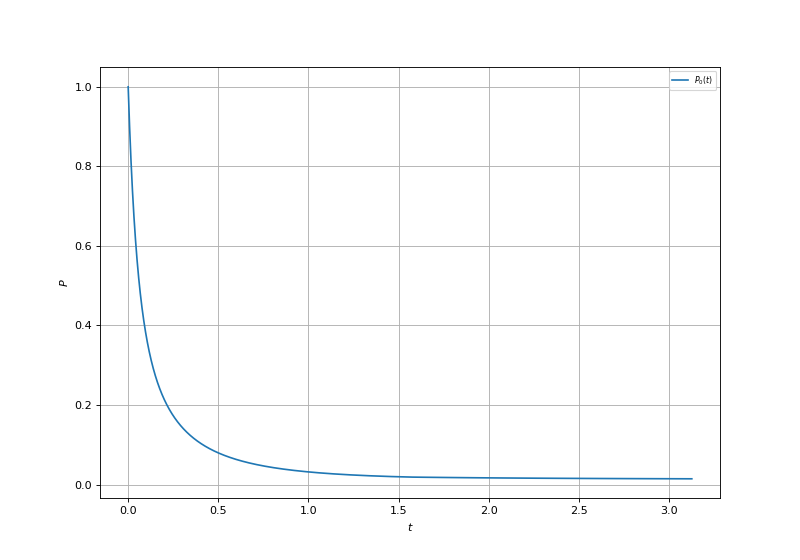
\includegraphics[width=\textwidth]{Images/P_o.png}}
\caption{Функция вероятности для 0 состояния}
\label{P_o}
\end{figure}

\begin{figure}[H]
\centerline{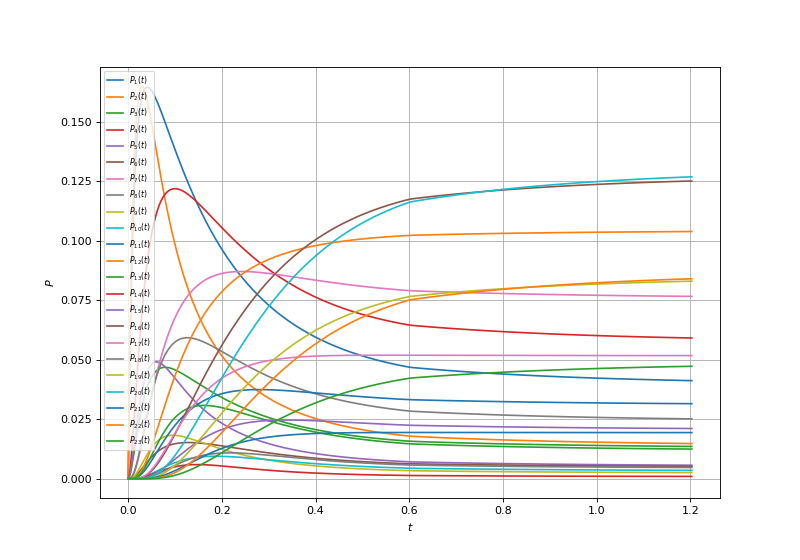
\includegraphics[width=\textwidth]{Images/P_i.png}}
\caption{Функции вероятностей для всех состояний (помимо 0) }
\label{P_i}
\end{figure}

\subsubsection{Прикладные характеристики системы}

Функция отказа может быть определена следующим образом:
$$1-R(t) = P_{term}(t)$$

График функции отказа $1-R(t)$ представлен на рисунке \ref{R_t}.
\begin{figure}[H]
\centerline{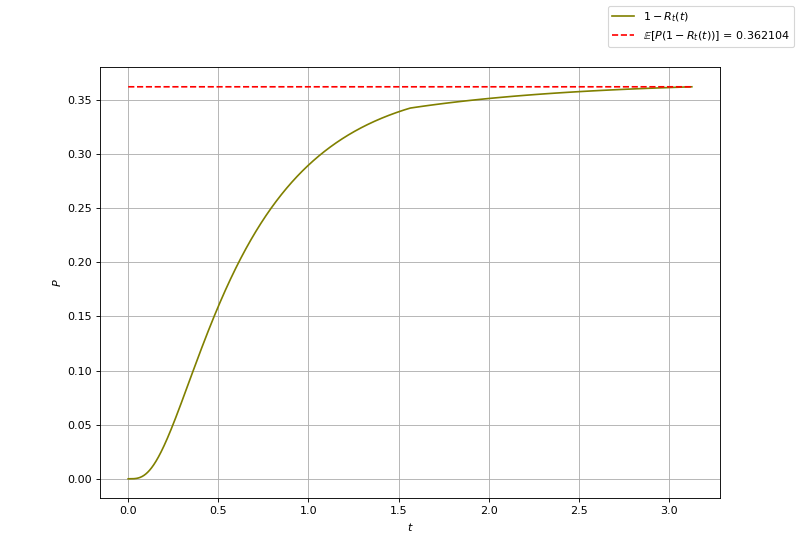
\includegraphics[width=\textwidth]{Images/R_t.png}}
\caption{Функция отказа системы}
\label{R_t}
\end{figure}

\begin{itemize}
    \item Математическое ожидание вероятности отказа:
$\mathbb{E}[P(1-R_t(t))]={{ mu }} $;
\item Коэффициент загрузки ремонтной службы: ${{ kzrs }}$;
\item Среднее число готовых к эксплуатации устройств типа  A и B: ${{ sngeA }}, {{ sngeB }}$ соответственно;
\end{itemize}

\subsubsection{Имитационное моделирование системы}

Для системы с непрерывным временем была реализована функция, осуществляющая переходы по состояниям.

\begin{lstlisting}[language=python, label=prog,caption={\textit{реализация марковского процесса}}]
# моделирование одного эпизода с непрерывным временем
def MD(m):
    current_s = 0
    current_t = 0
    states_tr = [current_s]
    t_tr = [0]
    times = np.zeros(len(m))
    last = np.zeros(len(m))

    while 1:
        l_b, l_a, l_s = find_lambda(m[current_s])
         # -log(1-y)/(lambda_a+lambda_b)
        t_cur_s = F_t(l_a[0] + l_b[0] + l_s[0],
                      np.random.uniform(low=0.0, high=1.0, size=None))

        times[current_s] += t_cur_s
        current_t += t_cur_s
        idx_b = l_b[1]
        idx_a = l_a[1]
        idx_s = l_s[1]
        current_s = np.random.choice([idx_a, idx_b, idx_s],
                                     p=[l_a[0] / (l_a[0] + l_b[0] + l_s[0]),
                                        l_b[0] / (l_a[0] + l_b[0] + l_s[0]),
                                        l_s[0] / (l_a[0] + l_b[0] + l_s[0])])
        # для дальнейшей отрисовки
        states_tr.append(current_s)
        t_tr.append(current_t)

        if distance.euclidean(times / current_t, last)<0.00001:
            return states_tr, t_tr, [np.mean(w_A), np.mean(w_B)], times / current_t, current_t

        last = times / current_t
\end{lstlisting}



На рисунке \ref{MDP} представлен график переключению состояний системы для 1 прогона ($N=1$).
\begin{figure}[H]
\centerline{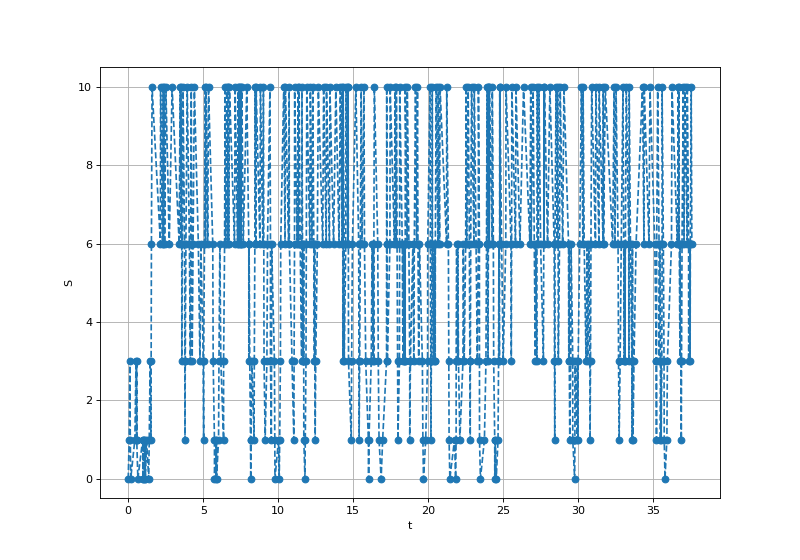
\includegraphics[width=\textwidth]{Images/term.png}}
\caption{График переключению состояний системы}
\label{MDP}
\end{figure}

Для $N=100$:
\begin{itemize}
    \item Среднее $t$ выхода на установившийся режим работы ${{ t_sr_v }}$;

    \item Статистические оценки предельных вероятностей после выхода на установившийся режим:
    \[
    \resizebox{\textwidth}{!}{$
[{{ p_pred_exp }}]
     $}
\]

\end{itemize}

\subsection{Дискретно-событийное моделирование системы}

Основные элементы дискретно-событийного моделирования системы:
\begin{itemize}
    \item Часы -- текущее "время" внутри моделирования.
    \item События -- поломка или починка устройства.
\end{itemize}
Блок-схема алгортима дискретно-событийного моделирования представлена на рисунке \ref{BS}

\begin{figure}[H]
\centerline{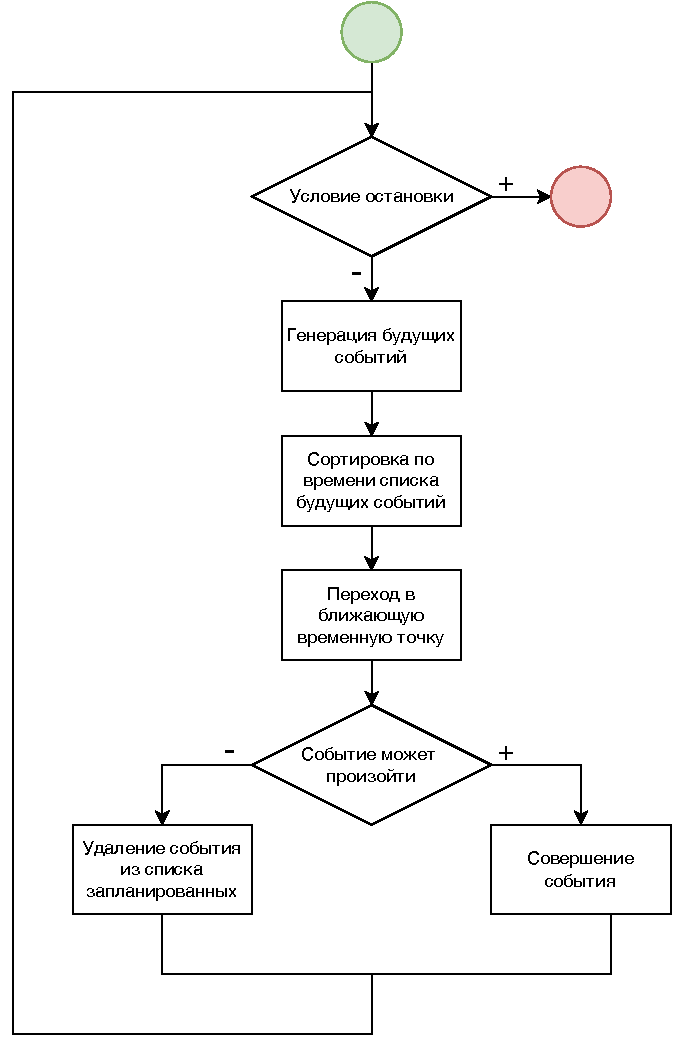
\includegraphics[width=0.5\textwidth]{Images/BS.pdf}}
\caption{Блок-схема алгоритма дискретно-событийного моделирования}
\label{BS}
\end{figure}

Результаты моделирования при $N=1$:
\scriptsize
\begin{verbatim}
{{ modeling_log }}
\end{verbatim}
\normalsize

Статистические данные при $N=100$:
\begin{itemize}
    \item Cреднее число готовых к эксплуатации устройств типа A и B = $ {{ t_sr_v_dsm[0] }}, {{ t_sr_v_dsm[1] }} $,
    \item Среднее время выхода в установившийся режим работы = $ {{ p_pred_exp_dsm }} $
\end{itemize}
%-------------------------------------------------
\subsection{Вывод}
В ходе выполнения домашнего задания была промоделирована работа СМО в терминах непрерывных марковских цепей,
а также выполнен анализ ее работы.

% --------------------------------------
% Атрибуты задачи
\labattributes{}{}{}{}{студент группы \EduGroup, \Author}{\Year, \Semestr}
%--------------

